\chapter{Os polímeros}\label{ch:g12:polymers}

Uma jaqueta de fleece pode ser fiada a partir de garrafas derretidas;
uma corda de escalada é feita de náilon; esta página é celulose,
fabricada pelas árvores. Os três são \omterm{def:g12:polymers:polymer}{polímeros}: \omterm{def:g7:atoms-and-molecules:molecule}{moléculas} com milhares
de \omterm{def:g7:atoms-and-molecules:atom}{átomos} de comprimento, construídas pela repetição, de novo e de novo,
de uma pequena unidade. As suas propriedades --- macio ou rígido,
elástico ou quebradiço, fundível ou não --- vêm menos dos \omterm{def:g7:atoms-and-molecules:atom}{átomos} que eles
contêm do que da maneira como as suas longas cadeias estão arrumadas.

\begin{recall}
Os \omterm{def:g8:plastics:plastic}{plásticos} são feitos de \omterm{def:g7:atoms-and-molecules:molecule}{moléculas} muito longas; os \omterm{def:g8:plastics:thermoplastic}{termoplásticos}
amolecem com o aquecimento, os \omterm{def:g8:plastics:thermoplastic}{termofixos} não
(\cref{ch:g8:plastics}). Os grupos \omterm{def:g11:functional-groups:alcohol}{álcool}, ácido, \omterm{def:g11:functional-groups:carboxylic-acid}{éster}, \omterm{def:g11:functional-groups:amine}{amina} e \omterm{def:g11:functional-groups:amine}{amida}
(\cref{ch:g11:functional-groups}). Uma adição junta duas \omterm{def:g7:atoms-and-molecules:molecule}{moléculas} numa
só sem perder nenhum \omterm{def:g7:atoms-and-molecules:atom}{átomo} (\cref{ch:g12:curly-arrows}).
\end{recall}

\begin{omfigure}
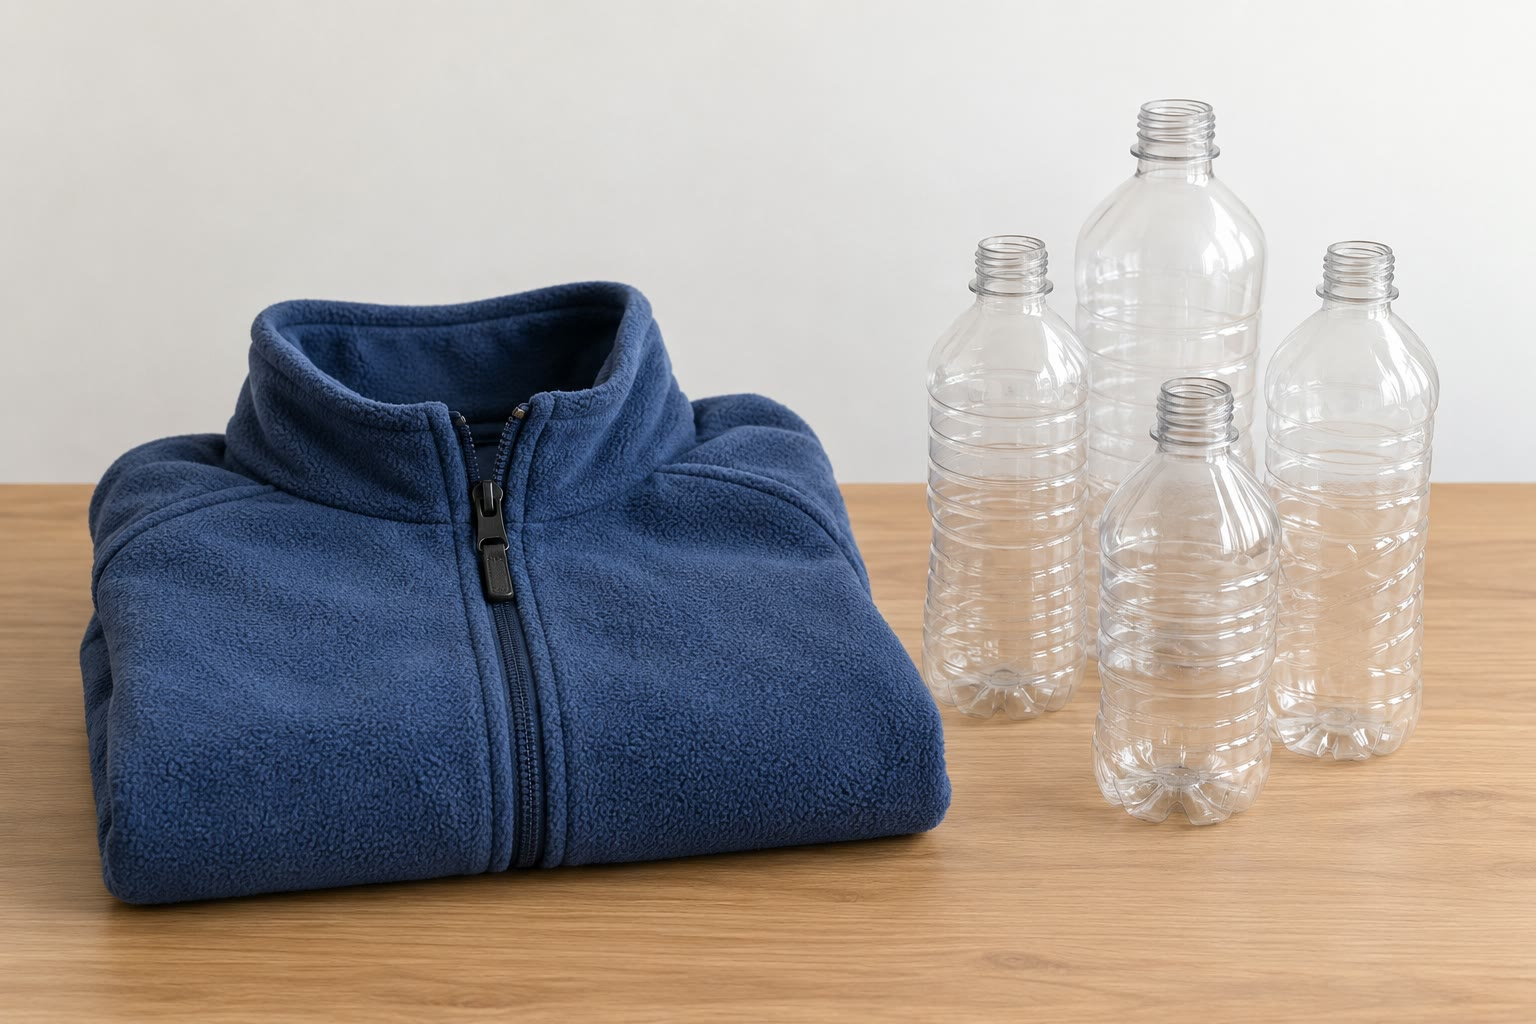
\includegraphics[width=0.45\linewidth]{images/book1/ai/g12-fleece-bottles.jpg}

{\small Garrafas usadas e uma jaqueta de fleece: o mesmo \omterm{def:g12:polymers:polymer}{polímero}, em duas
formas.}
\end{omfigure}

\section{Monômeros, polímeros, unidades de repetição}

\begin{definition}[Polímero, monômero, polimerização]\label{def:g12:polymers:polymer}
Um \emph{polímero}\index{polimero@polímero} é uma substância feita de \omterm{def:g7:atoms-and-molecules:molecule}{moléculas}
muito grandes, as macromoléculas, cada uma construída a partir de muitas
pequenas unidades ligadas umas atrás das outras. As pequenas \omterm{def:g7:atoms-and-molecules:molecule}{moléculas} a
partir das quais ele é feito são os seus
\emph{monômeros}\index{monomero@monômero}; a reação que as junta é uma
\emph{polimerização}\index{polimerizacao@polimerização}.
\end{definition}

\begin{definition}[Unidade de repetição, grau de polimerização]\label{def:g12:polymers:repeat-unit}
A \emph{unidade de repetição}\index{unidade de repeticao@unidade de repetição} de um \omterm{def:g12:polymers:polymer}{polímero}
é o menor grupo de \omterm{def:g7:atoms-and-molecules:atom}{átomos} cuja repetição dá a cadeia; ela é escrita
entre colchetes com um \omterm{def:g7:atoms-and-molecules:formula}{índice} $n$. O número $n$ de unidades de repetição
de uma cadeia é o seu \emph{grau de
polimerização}\index{grau de polimerizacao@grau de polimerização}.
\end{definition}
\begin{omfigure}
\[
  n\;\ce{CH2=CH2}
  \quad\longrightarrow\quad
  \chemfig{-[@{op1,.75}]CH_2-CH_2-[@{cl1,0.25}]}
  \polymerdelim[height=6pt, depth=6pt, indice=n]{op1}{cl1}
\]

{\small A \omterm{def:g12:polymers:polymer}{polimerização} do eteno: $n$ \omterm{def:g7:atoms-and-molecules:molecule}{moléculas} de \omterm{def:g12:polymers:polymer}{monômero} dão uma
cadeia de polietileno, cuja \omterm{def:g12:polymers:repeat-unit}{unidade de repetição} \ce{-CH2-CH2-} é
escrita entre colchetes.}
\end{omfigure}

\begin{proposition}[A massa molar de um polímero]\label{prop:g12:polymers:molar-mass}
Uma cadeia de \omterm{def:g12:polymers:repeat-unit}{grau de polimerização} $n$ tem uma \omterm{def:g10:the-mole:molar-mass}{massa molar}
\[
  M(\text{polímero}) \approx n \times M(\text{unidade de repetição}) ,
\]
já que as duas pontas da cadeia são desprezíveis para $n$ grande.
\end{proposition}

\begin{proof}
A cadeia é formada por $n$ \omterm{def:g12:polymers:repeat-unit}{unidades de repetição} mais dois grupos
terminais de alguns \omterm{def:g7:atoms-and-molecules:atom}{átomos} cada; para $n$ na casa dos milhares, os
grupos terminais pesam menos de um milésimo do total.
\end{proof}

\begin{example}[Uma cadeia de polietileno]\label{ex:g12:polymers:pe}
% ledger: aw:C, aw:H
Uma cadeia de polietileno de \omterm{def:g10:the-mole:molar-mass}{massa molar} \qty{280000}{g/mol} tem
$n = 280000/28.0 = 10000$ \omterm{def:g12:polymers:repeat-unit}{unidades de repetição}, isto é, vinte mil
\omterm{def:g7:atoms-and-molecules:atom}{átomos} de carbono em fila. Numa amostra real, as cadeias não têm todas o
mesmo comprimento: $n$ é uma média.
\end{example}

\section{Os polímeros de adição}

\begin{definition}[Polímero de adição, polímero de condensação]\label{def:g12:polymers:addition-polymer}
Um \emph{polímero de adição}\index{polimero de adicao@polímero de adição} se forma por
adições de \omterm{def:g12:polymers:polymer}{monômeros} que carregam uma \omterm{def:g10:lewis-and-shape:multiple-bond}{ligação dupla} \ce{C=C}, sem nenhum
outro produto: a sua \omterm{def:g12:polymers:repeat-unit}{unidade de repetição} tem os mesmos \omterm{def:g7:atoms-and-molecules:atom}{átomos} que o
\omterm{def:g12:polymers:polymer}{monômero}. Um \emph{polímero de
condensação}\index{polimero de condensacao@polímero de condensação} se forma por reações entre
dois \omterm{def:g11:functional-groups:functional-group}{grupos funcionais} que juntam dois \omterm{def:g12:polymers:polymer}{monômeros} e liberam uma \omterm{def:g7:atoms-and-molecules:molecule}{molécula}
pequena, em geral água, a cada ligação.
\end{definition}

\begin{omfigure}
\footnotesize
\renewcommand{\arraystretch}{1.5}
\begin{tabular}{l l l l}
\hline
\omterm{def:g12:polymers:polymer}{monômero} & \omterm{def:g12:polymers:polymer}{polímero} & \omterm{def:g12:polymers:repeat-unit}{unidade de repetição} & usos \\
\hline
eteno \ce{CH2=CH2} & polietileno (PE) & \ce{-CH2-CH2-} & sacolas, garrafas \\
cloroeteno \ce{CH2=CHCl} & poli(cloreto de vinila) (PVC) & \ce{-CH2-CHCl-} & canos, esquadrias \\
fenileteno \ce{CH2=CH-C6H5} & poliestireno (PS) & \ce{-CH2-CH(C6H5)-} & copos, isopor \\
tetrafluoroeteno \ce{CF2=CF2} & PTFE & \ce{-CF2-CF2-} & panelas antiaderentes \\
\hline
\end{tabular}\par\medskip

{\small Quatro \omterm{def:g12:polymers:addition-polymer}{polímeros de adição}. Em cada um, a \omterm{def:g10:lewis-and-shape:multiple-bond}{ligação dupla} do
\omterm{def:g12:polymers:polymer}{monômero} se abre, e os seus dois carbonos entram na cadeia.}
\end{omfigure}

\begin{method}[Encontrar o monômero a partir de um polímero]\label{met:g12:polymers:monomer}
\begin{enumerate}
  \item Encontre a \omterm{def:g12:polymers:repeat-unit}{unidade de repetição}: o menor grupo cuja repetição dá
        a cadeia.
  \item Se a cadeia principal só contém \omterm{def:g7:atoms-and-molecules:atom}{átomos} de carbono, é um \omterm{def:g12:polymers:addition-polymer}{polímero
        de adição}: recoloque uma \omterm{def:g10:lewis-and-shape:multiple-bond}{ligação dupla} entre os dois carbonos da
        cadeia principal da \omterm{def:g12:polymers:repeat-unit}{unidade de repetição}. Esse é o \omterm{def:g12:polymers:polymer}{monômero}.
  \item Se a cadeia principal contém ligações \omterm{def:g11:functional-groups:carboxylic-acid}{éster} ou \omterm{def:g11:functional-groups:amine}{amida}, é um
        \omterm{def:g12:polymers:addition-polymer}{polímero de condensação}: corte cada ligação, e devolva a cada
        lado os \omterm{def:g7:atoms-and-molecules:atom}{átomos} da \omterm{def:g7:atoms-and-molecules:molecule}{molécula} pequena liberada (\ce{-OH} ao
        \ce{C=O}, \ce{-H} ao \ce{O} ou ao \ce{N}). Esses são os
        \omterm{def:g12:polymers:polymer}{monômeros}.
\end{enumerate}
\end{method}

\begin{example}[O monômero do PVC]\label{ex:g12:polymers:pvc}
A cadeia \ce{-CH2-CHCl-CH2-CHCl-CH2-CHCl-} repete \ce{-CH2-CHCl-}; ela
só contém carbonos na cadeia principal, logo o \omterm{def:g12:polymers:polymer}{monômero} é
\ce{CH2=CHCl}, o cloroeteno.
\end{example}

\section{Os polímeros de condensação}

Um \omterm{def:g12:polymers:polymer}{monômero} com um só grupo reativo só pode se ligar uma vez: ele
termina uma cadeia. Para construir uma cadeia por condensação, cada
\omterm{def:g12:polymers:polymer}{monômero} precisa de dois grupos, um em cada ponta.

\begin{example}[O PET, um poliéster]\label{ex:g12:polymers:pet}
% ledger: aw:C, aw:H, aw:O
O etano-1,2-diol, \ce{HO-CH2-CH2-OH}, carrega dois grupos \omterm{def:g11:functional-groups:alcohol}{álcool}; o
ácido benzeno-1,4-dicarboxílico, \ce{HOOC-C6H4-COOH}, dois grupos ácido.
Cada grupo ácido forma um \omterm{def:g11:functional-groups:carboxylic-acid}{éster} com um grupo \omterm{def:g11:functional-groups:alcohol}{álcool} e libera água: a
cadeia cresce pelas duas pontas. O \omterm{def:g12:polymers:polymer}{polímero} é o poli(tereftalato de
etileno), o PET, o material das garrafas de bebida e das fibras de
poliéster. A sua \omterm{def:g12:polymers:repeat-unit}{unidade de repetição}, \ce{C10H8O4}, tem uma \omterm{def:g10:the-mole:molar-mass}{massa molar}
de \qty{192.0}{g/mol}, isto é, os dois \omterm{def:g12:polymers:polymer}{monômeros} ($62.0 + 166.0$) menos
duas \omterm{def:g7:atoms-and-molecules:molecule}{moléculas} de água ($36.0$).
\end{example}

\begin{omfigure}
\setchemfig{atom sep=1.9em}
\chemfig{HO-CH_2-CH_2-OH}
\quad $+$ \quad
\chemfig{HO-C(=[2]O)-*6(-=-(-C(=[2]O)-OH)=-=)}

\medskip
$\longrightarrow$\quad
\chemfig{-[@{op2,.75}]O-CH_2-CH_2-O-C(=[2]O)-*6(-=-(-C(=[2]O)-[@{cl2,0.25}])=-=)}
\polymerdelim[height=20pt, depth=6pt, indice=n]{op2}{cl2}
\quad $+\ 2n\ \ce{H2O}$

{\small O PET a partir dos seus dois \omterm{def:g12:polymers:polymer}{monômeros}: cada ligação \omterm{def:g11:functional-groups:carboxylic-acid}{éster} (os
grupos \ce{-CO-O-}) libera uma \omterm{def:g7:atoms-and-molecules:molecule}{molécula} de água.}
\end{omfigure}

\begin{example}[O náilon-6,6, uma poliamida]\label{ex:g12:polymers:nylon}
A hexano-1,6-diamina, \ce{H2N-(CH2)6-NH2}, e o ácido hexanodioico,
\ce{HOOC-(CH2)4-COOH}, se juntam por ligações \omterm{def:g11:functional-groups:amine}{amida}, cada uma liberando
uma \omterm{def:g7:atoms-and-molecules:molecule}{molécula} de água:
\[
  \cdots\ce{-NH-(CH2)6-NH-CO-(CH2)4-CO-}\cdots
\]
Os dois seis do nome contam os \omterm{def:g7:atoms-and-molecules:atom}{átomos} de carbono de cada \omterm{def:g12:polymers:polymer}{monômero}. As
ligações \omterm{def:g11:functional-groups:amine}{amida} de cadeias vizinhas se atraem por \omterm{def:g11:polarity-and-cohesion:hydrogen-bond}{ligações de hidrogênio},
o que torna as fibras de náilon resistentes.
\end{example}

\begin{history}[Carothers e o náilon]
% ledger: hist:polyamides-1934, hist:nylon-production-1939
O químico Wallace Carothers, que dirigia um laboratório de pesquisa de
uma empresa química, decidiu provar que os \omterm{def:g12:polymers:polymer}{polímeros} eram verdadeiras
\omterm{def:g7:atoms-and-molecules:molecule}{moléculas} gigantes e fabricá-los de propósito. A sua equipe fez primeiro
poliésteres, que fundiam fácil demais para serem úteis; em 1934, ela se
voltou para as \omterm{def:g11:functional-groups:amine}{aminas} e fez poliamidas, entre elas a fibra que mais
tarde recebeu o nome de náilon. O náilon entrou em produção em 1939,
primeiro como meias que causaram sensação numa Feira Mundial, depois
como paraquedas, cordas e cerdas de escova de dentes.
\end{history}

\begin{omfigure}
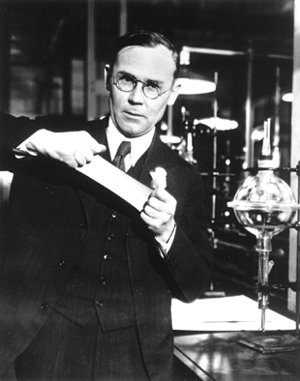
\includegraphics[width=0.24\linewidth]{images/book1/carothers.jpg}

{\small Wallace Carothers no seu laboratório.}
\end{omfigure}

\section{Estrutura e propriedades}

Duas amostras do mesmo \omterm{def:g12:polymers:polymer}{polímero} podem se comportar de maneiras muito
diferentes: o que conta é o comprimento das cadeias, a sua forma e a
maneira como elas estão arrumadas.

\begin{proposition}[Cadeias e propriedades]\label{prop:g12:polymers:properties}
\begin{itemize}
  \item Cadeias mais longas se emaranham mais: o material é mais
        resistente e funde a uma temperatura mais alta.
  \item Cadeias lineares podem se alinhar lado a lado em regiões
        ordenadas, \emph{cristalinas}; cadeias ramificadas não podem, e
        ficam desordenadas, \emph{amorfas}. As regiões cristalinas
        tornam um \omterm{def:g12:polymers:polymer}{polímero} mais denso, mais rígido e menos transparente.
  \item Cadeias mantidas lado a lado só por forças intermoleculares
        deslizam umas sobre as outras quando aquecidas: o \omterm{def:g12:polymers:polymer}{polímero} é um
        \omterm{def:g8:plastics:thermoplastic}{termoplástico}. Cadeias unidas por \emph{ligações cruzadas}
        covalentes não podem: o \omterm{def:g12:polymers:polymer}{polímero} é um \omterm{def:g8:plastics:thermoplastic}{termofixo} ou, com poucas
        ligações cruzadas, um sólido elástico como a borracha.
\end{itemize}
\end{proposition}

\begin{proof}
O aquecimento dá às cadeias energia suficiente para vencer as forças
intermoleculares entre elas (\cref{ch:g11:polarity-and-cohesion}), que
são mais fracas que as \omterm{def:g10:lewis-and-shape:covalent-bond}{ligações covalentes}; quanto mais contato entre as
cadeias, mais energia isso exige. As ligações cruzadas são covalentes:
rompê-las destrói o material em vez de fundi-lo.
\end{proof}

\begin{omfigure}
\begin{tikzpicture}[font=\footnotesize, line width=1pt, line cap=round,
    lab/.style={below, align=center, text width=2.8cm}]
  % linear, packed (crystalline)
  \begin{scope}
    \foreach \y in {0,0.25,0.5,0.75,1.0}
      \draw[omDef] plot[smooth, domain=0:2.2, samples=25] (\x, {\y + 0.05*sin(400*\x)});
    \node[lab] at (1.1,-0.2) {cadeias lineares\\ alinhadas: cristalinas};
  \end{scope}
  % linear, tangled (amorphous)
  \begin{scope}[xshift=3.4cm]
    \draw[omDef] plot[smooth] coordinates {(0,0.2) (0.5,0.9) (1.0,0.3) (1.4,1.1) (2.0,0.5) (2.2,0.9)};
    \draw[omProp] plot[smooth] coordinates {(0,0.9) (0.4,0.3) (0.9,1.0) (1.5,0.2) (1.9,1.0) (2.2,0.3)};
    \draw[black!60] plot[smooth] coordinates {(0.1,0.55) (0.7,0.1) (1.2,0.75) (1.7,0.55) (2.2,0.1)};
    \node[lab] at (1.1,-0.2) {cadeias lineares\\ emaranhadas: amorfas};
  \end{scope}
  % branched
  \begin{scope}[xshift=6.8cm]
    \draw[omDef] plot[smooth] coordinates {(0,0.5) (0.6,0.6) (1.2,0.45) (1.8,0.65) (2.2,0.5)};
    \draw[omDef] (0.5,0.6) -- (0.35,1.05) (1.0,0.5) -- (1.15,0.05) (1.6,0.6) -- (1.5,1.1) (1.6,0.6) -- (1.95,1.0);
    \node[lab] at (1.1,-0.2) {cadeias ramificadas:\\ não se arrumam};
  \end{scope}
  % cross-linked
  \begin{scope}[xshift=10.2cm]
    \foreach \y in {0.1,0.55,1.0}
      \draw[omDef] plot[smooth, domain=0:2.2, samples=25] (\x, {\y + 0.06*sin(300*\x)});
    \foreach \x/\a/\b in {0.4/0.1/0.55, 1.3/0.1/0.55, 0.9/0.55/1.0, 1.9/0.55/1.0}
      \draw[omProp, line width=1.6pt] (\x,\a) -- (\x,\b);
    \node[lab] at (1.1,-0.2) {cadeias com ligações\\ cruzadas: não fundem};
  \end{scope}
\end{tikzpicture}

{\small Quatro arranjos de cadeias de \omterm{def:g12:polymers:polymer}{polímero}. As ligações cruzadas (em
laranja) são \omterm{def:g10:lewis-and-shape:covalent-bond}{ligações covalentes} entre cadeias.}
\end{omfigure}

\begin{example}[Dois polietilenos]\label{ex:g12:polymers:two-pe}
O polietileno fabricado sob pressão muito alta tem muitas ramificações
curtas: as suas cadeias se arrumam mal, e ele dá filmes macios e
transparentes para sacolas. Fabricado com um \omterm{def:g12:catalysis:catalyst}{catalisador} a baixa
pressão, as suas cadeias são quase lineares e se arrumam em regiões
cristalinas: ele é mais denso e mais rígido, e dá garrafas de leite e
engradados. O mesmo \omterm{def:g12:polymers:polymer}{monômero}, a mesma \omterm{def:g12:polymers:repeat-unit}{unidade de repetição}, uma
arquitetura diferente.
\end{example}

\section{Os polímeros naturais}

Os seres vivos fabricaram \omterm{def:g12:polymers:polymer}{polímeros} muito antes dos químicos.

\begin{itemize}
  \item A \textbf{celulose} e o \textbf{amido} são ambos cadeias de
        unidades de glicose, \ce{C6H10O5} por unidade, ligadas de modo
        diferente: a celulose forma fibras retas e resistentes (madeira,
        algodão, papel); o amido forma espirais que o organismo digere.
  \item As \textbf{proteínas} são cadeias de aminoácidos unidos por
        ligações \omterm{def:g11:functional-groups:amine}{amida}, as ligações peptídicas do dipeptídeo do
        \cref{ch:g12:synthesis-strategy}.
  \item O \textbf{DNA} é uma cadeia de nucleotídeos; a ordem dos seus
        quatro tipos de unidade armazena a informação genética.
  \item A \textbf{borracha natural} é um \omterm{def:g12:polymers:addition-polymer}{polímero de adição} do isopreno,
        \ce{CH2=C(CH3)-CH=CH2}, recolhido como um líquido leitoso, o
        látex, da casca da seringueira. Aquecida com enxofre, as suas
        cadeias são ligadas por pontes de enxofre: a borracha fica mais
        resistente e conserva a sua forma, como num pneu.
\end{itemize}

\begin{omfigure}
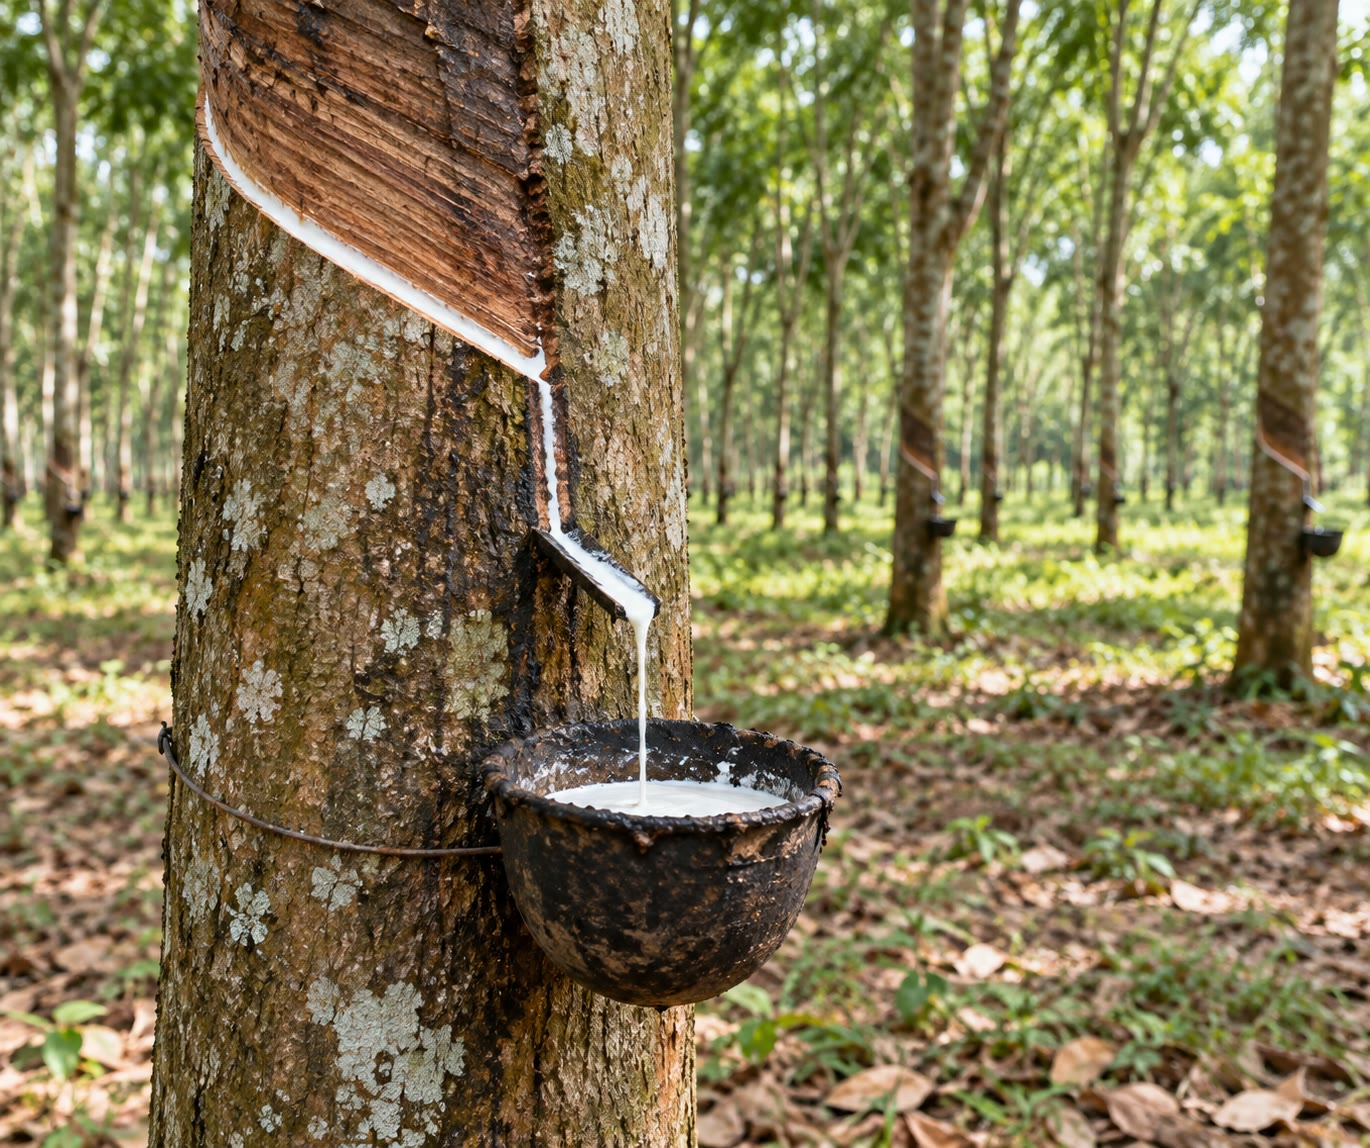
\includegraphics[width=0.45\linewidth]{images/book1/ai/g12-rubber-tapping.jpg}

{\small A sangria de uma seringueira: o látex escorre de um corte na
casca para dentro de uma tigela.}
\end{omfigure}

\begin{remark}[Fazer e desfazer]\label{rem:g12:polymers:recycling}
Um \omterm{def:g8:plastics:thermoplastic}{termoplástico} pode ser fundido e moldado de novo: é a \omterm{def:g5:raw-materials-and-recycling:recycling}{reciclagem}
mecânica. Um \omterm{def:g12:polymers:addition-polymer}{polímero de condensação} também pode ser quebrado nos seus
\omterm{def:g12:polymers:polymer}{monômeros} pela reação inversa, uma hidrólise, e os \omterm{def:g12:polymers:polymer}{monômeros}
transformados em novo \omterm{def:g12:polymers:polymer}{polímero}: é a \omterm{def:g5:raw-materials-and-recycling:recycling}{reciclagem} química. Um \omterm{def:g8:plastics:thermoplastic}{termofixo} não
se presta facilmente a nenhuma das duas.
\end{remark}

\section{Exercícios}

\begin{exercise}[$\star$]\label{exo:g12:polymers:1}
Dê o \omterm{def:g12:polymers:polymer}{monômero} do polipropileno, cuja \omterm{def:g12:polymers:repeat-unit}{unidade de repetição} é
\ce{-CH2-CH(CH3)-}.
\end{exercise}

\begin{exercise}[$\star$]\label{exo:g12:polymers:2}
Escreva a \omterm{def:g12:polymers:repeat-unit}{unidade de repetição} do \omterm{def:g12:polymers:polymer}{polímero} fabricado a partir do
tetrafluoroeteno, \ce{CF2=CF2}. É um \omterm{def:g12:polymers:addition-polymer}{polímero de adição} ou de
condensação?
\end{exercise}

\begin{exercise}[$\star$]\label{exo:g12:polymers:3}
Classifique como \omterm{def:g12:polymers:addition-polymer}{polímeros de adição} ou de condensação: polietileno,
PET, náilon, PVC, poliestireno.
\end{exercise}

\begin{exercise}[$\star$]\label{exo:g12:polymers:4}
Quais destes \omterm{def:g12:polymers:polymer}{polímeros} são naturais: celulose, náilon, amido, PVC,
borracha de látex, proteínas?
\end{exercise}

\begin{exercise}[$\star$]\label{exo:g12:polymers:5}
Por que cada \omterm{def:g12:polymers:polymer}{monômero} de um \omterm{def:g12:polymers:addition-polymer}{polímero de condensação} deve carregar dois
grupos reativos?
\end{exercise}

\begin{exercise}[$\star\star$]\label{exo:g12:polymers:6}
Uma amostra de PVC tem uma \omterm{def:g10:the-mole:molar-mass}{massa molar} média de \qty{125000}{g/mol}.
Calcule o seu \omterm{def:g12:polymers:repeat-unit}{grau de polimerização}.
\end{exercise}

\begin{exercise}[$\star\star$]\label{exo:g12:polymers:7}
Uma cadeia de poliestireno tem um \omterm{def:g12:polymers:repeat-unit}{grau de polimerização} de 2500. Calcule
a sua \omterm{def:g10:the-mole:molar-mass}{massa molar}.
\end{exercise}

\begin{exercise}[$\star\star$]\label{exo:g12:polymers:8}
O ácido lático, \ce{CH3-CH(OH)-COOH}, carrega um grupo \omterm{def:g11:functional-groups:alcohol}{álcool} e um grupo
ácido. Mostre que ele pode formar sozinho um poliéster, escreva a sua
\omterm{def:g12:polymers:repeat-unit}{unidade de repetição} e dê o nome da \omterm{def:g7:atoms-and-molecules:molecule}{molécula} pequena liberada.
\end{exercise}

\begin{exercise}[$\star\star$]\label{exo:g12:polymers:9}
Explique, com a figura dos arranjos de cadeias, por que os filmes de
sacola são macios e transparentes, enquanto as garrafas de leite são
rígidas e opacas.
\end{exercise}

\begin{exercise}[$\star\star$]\label{exo:g12:polymers:10}
O cabo de uma panela é um \omterm{def:g8:plastics:thermoplastic}{termofixo}, e o pegador de \omterm{def:g8:plastics:plastic}{plástico} da tampa
também. Descreva as suas cadeias. Por que eles não podem ser fundidos e
reciclados?
\end{exercise}

\begin{exercise}[$\star\star$]\label{exo:g12:polymers:11}
Uma cadeia de náilon-6,6 tem uma \omterm{def:g10:the-mole:molar-mass}{massa molar} de \qty{22600}{g/mol}.
Calcule a \omterm{def:g10:the-mole:molar-mass}{massa molar} da sua \omterm{def:g12:polymers:repeat-unit}{unidade de repetição} \ce{C12H22N2O2}, e
depois o seu \omterm{def:g12:polymers:repeat-unit}{grau de polimerização}.
\end{exercise}

\begin{exercise}[$\star\star\star$]\label{exo:g12:polymers:12}
Escreva a reação entre uma \omterm{def:g7:atoms-and-molecules:molecule}{molécula} de hexano-1,6-diamina e uma de ácido
hexanodioico, que dá a primeira ligação \omterm{def:g11:functional-groups:amine}{amida}. Por que o produto pode
continuar reagindo pelas duas pontas?
\end{exercise}

\begin{exercise}[$\star\star\star$]\label{exo:g12:polymers:13}
Que massa de água é liberada quando se fabrica \qty{1.0}{kg} de
náilon-6,6?
\end{exercise}

\begin{exercise}[$\star\star\star$]\label{exo:g12:polymers:14}
A borracha natural é macia e pegajosa quando está quente; aquecida com
enxofre, ela vira a borracha elástica e resistente dos pneus. Explique
com as cadeias. Por que um pneu é tão difícil de reciclar?
\end{exercise}

\begin{exercise}[$\star\star\star$]\label{exo:g12:polymers:15}
O amido e a celulose têm a mesma fórmula por unidade, \ce{C6H10O5}. Uma
cadeia de celulose tem uma \omterm{def:g10:the-mole:molar-mass}{massa molar} de \qty{1.6e6}{g/mol}. Quantas
unidades de glicose ela contém? Qual é o seu comprimento, se cada
unidade acrescenta \qty{0.5}{nm} a ele?
\end{exercise}

\section{Problema: da garrafa ao fleece}

\begin{problem}[{Problema de fim de semana --- quantas garrafas de 25 g
cabem numa jaqueta de fleece?}]
\label{pb:g12:polymers:1}
% ledger: aw:C, aw:H, aw:O
Uma jaqueta de fleece é feita de \qty{300}{g} de fibra de PET. Garrafas
usadas de \qty{25}{g} cada são recolhidas, triadas, lavadas, trituradas,
fundidas e fiadas; nesse processo, \qty{80}{\percent} da massa das
garrafas acaba como fibra na jaqueta.

\medskip
\noindent\textbf{Parte I --- O \omterm{def:g12:polymers:polymer}{polímero}.}
\begin{enumerate}
  \item Dê o nome dos dois \omterm{def:g12:polymers:polymer}{monômeros} do PET e dos \omterm{def:g11:functional-groups:functional-group}{grupos funcionais} que
        eles carregam.
  \item Que ligação se forma entre eles? Que \omterm{def:g7:atoms-and-molecules:molecule}{molécula} pequena é
        liberada?
  \item O PET é um \omterm{def:g12:polymers:addition-polymer}{polímero de adição} ou de condensação?
  \item Calcule as \omterm{def:g10:the-mole:molar-mass}{massas molares} dos dois \omterm{def:g12:polymers:polymer}{monômeros}.
  \item Deduza a \omterm{def:g10:the-mole:molar-mass}{massa molar} da \omterm{def:g12:polymers:repeat-unit}{unidade de repetição} \ce{C10H8O4}, e
        confira-a com a sua fórmula.
\end{enumerate}

\medskip
\noindent\textbf{Parte II --- As cadeias.}
\begin{enumerate}[resume]
  \item O PET de uma garrafa tem cadeias de \omterm{def:g10:the-mole:molar-mass}{massa molar} média
        \qty{38400}{g/mol}. Calcule o \omterm{def:g12:polymers:repeat-unit}{grau de polimerização}.
  \item Quantas ligações \omterm{def:g11:functional-groups:carboxylic-acid}{éster} uma cadeia contém, aproximadamente?
  \item O PET das garrafas é em parte cristalino. O que isso diz sobre
        as suas cadeias?
  \item Por que o PET pode ser fundido e fiado como fibra?
\end{enumerate}

\medskip
\noindent\textbf{Parte III --- A \omterm{def:g5:raw-materials-and-recycling:recycling}{reciclagem}.}
\begin{enumerate}[resume]
  \item Que massa de garrafas é necessária para uma jaqueta?
  \item Quantas garrafas são isso?
  \item O que acontece com o resto da massa?
  \item Que princípio da \omterm{def:g12:synthesis-strategy:green-chemistry}{química verde} essa \omterm{def:g5:raw-materials-and-recycling:recycling}{reciclagem} aplica?
\end{enumerate}

\medskip
\noindent\textbf{Parte IV --- De volta aos \omterm{def:g12:polymers:polymer}{monômeros}.}
\begin{enumerate}[resume]
  \item Escreva, para uma \omterm{def:g12:polymers:repeat-unit}{unidade de repetição}, a hidrólise do PET nos
        seus \omterm{def:g12:polymers:polymer}{monômeros}.
  \item Que \omterm{def:g10:the-mole:amount}{quantidade de matéria} de \omterm{def:g12:polymers:repeat-unit}{unidades de repetição} há em
        \qty{1.00}{kg} de PET?
  \item Que massas de cada \omterm{def:g12:polymers:polymer}{monômero} dá a hidrólise completa de
        \qty{1.00}{kg} de PET?
  \item Que massa de água ela consome? Verifique a \omterm{def:g8:balanced-equations:conservation}{conservação da massa}.
  \item Dê uma vantagem dessa \omterm{def:g5:raw-materials-and-recycling:recycling}{reciclagem} química sobre a fusão.
  \item Dê a resposta final: quantas garrafas de \qty{25}{g} cabem numa
        jaqueta de fleece?
\end{enumerate}
\end{problem}
